\section{数据检索}
%%%% 初识网站 -------------------------------------------------------------------
\subsection{打开网站}
\begin{frame}{打开浏览器}
    打开一个非IE浏览器,以火狐为例。
    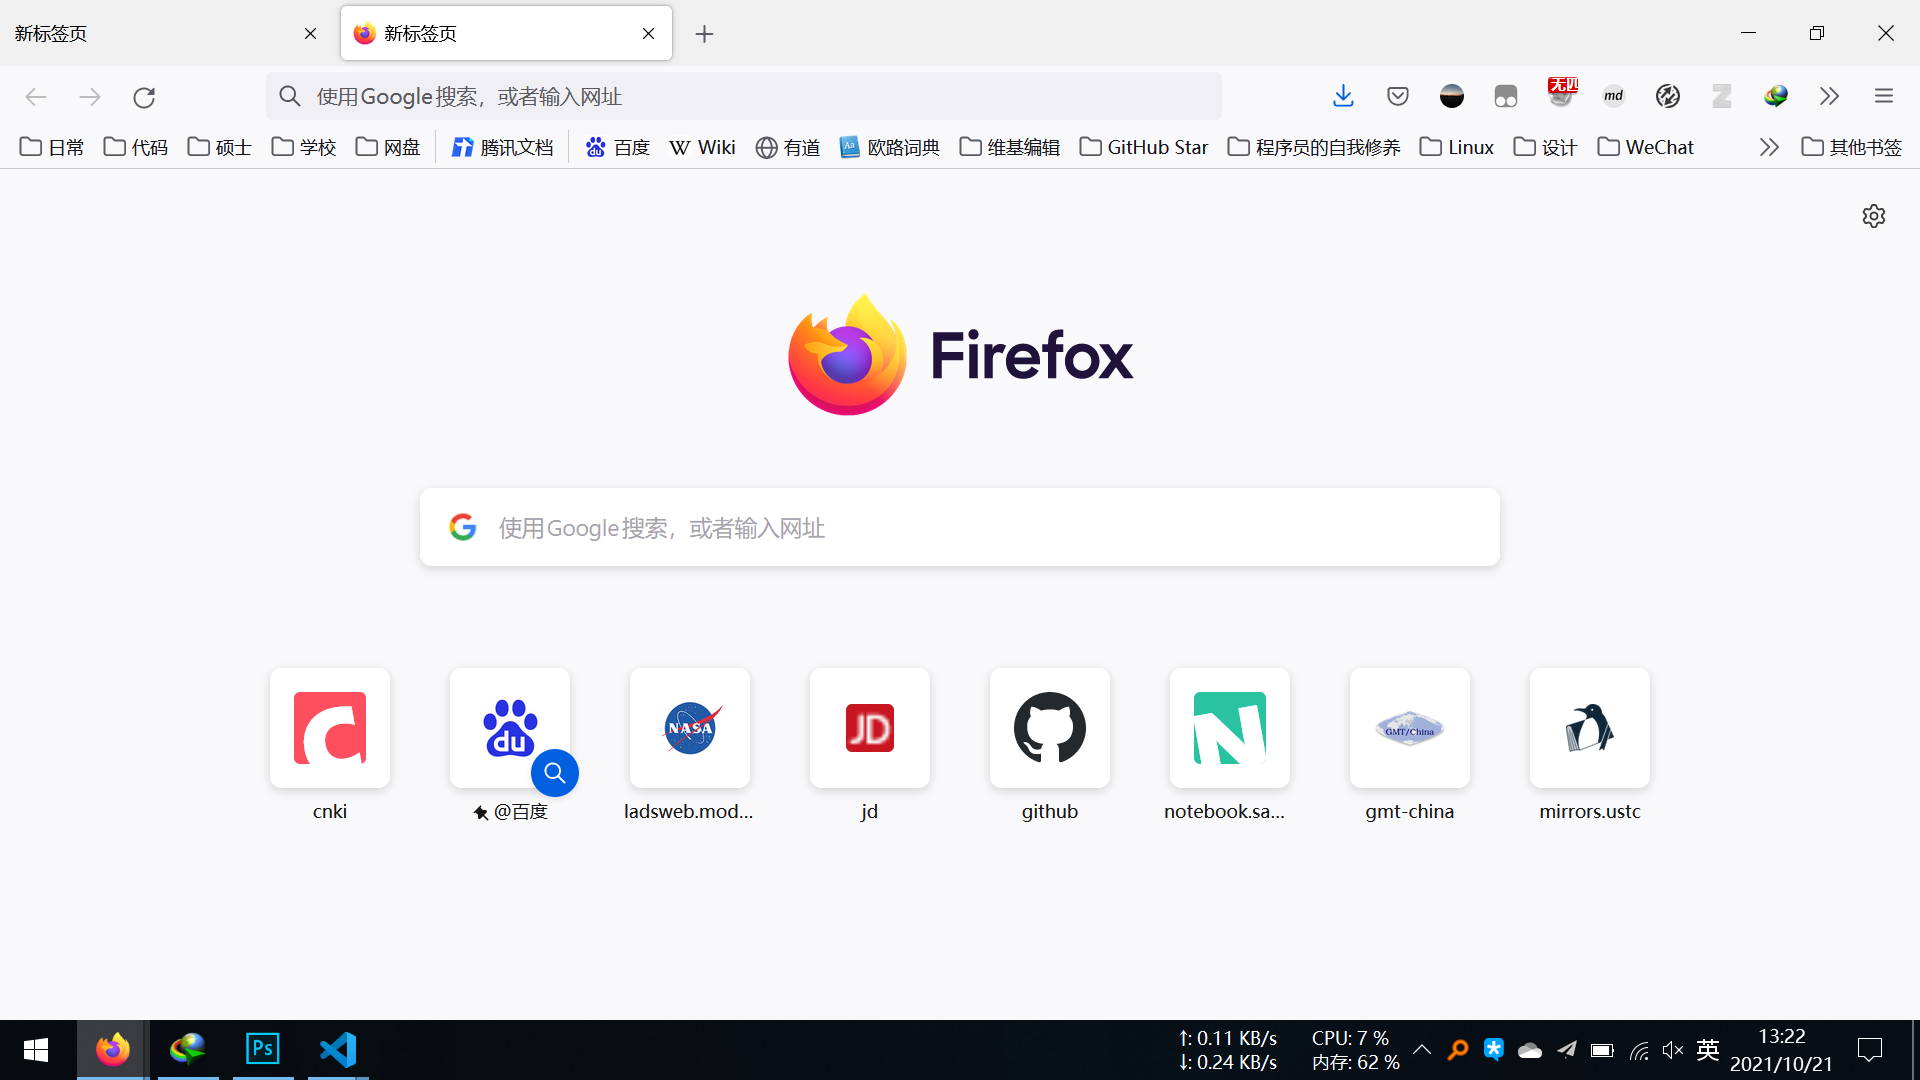
\includegraphics[width=\linewidth]{images/1.打开浏览器.png}
\end{frame}
\begin{frame}
    \frametitle{输入LAADS网址}
    输入网址\url{https://ladsweb.modaps.eosdis.nasa.gov/}

    按键盘上的Enter键或鼠标点击访问。
    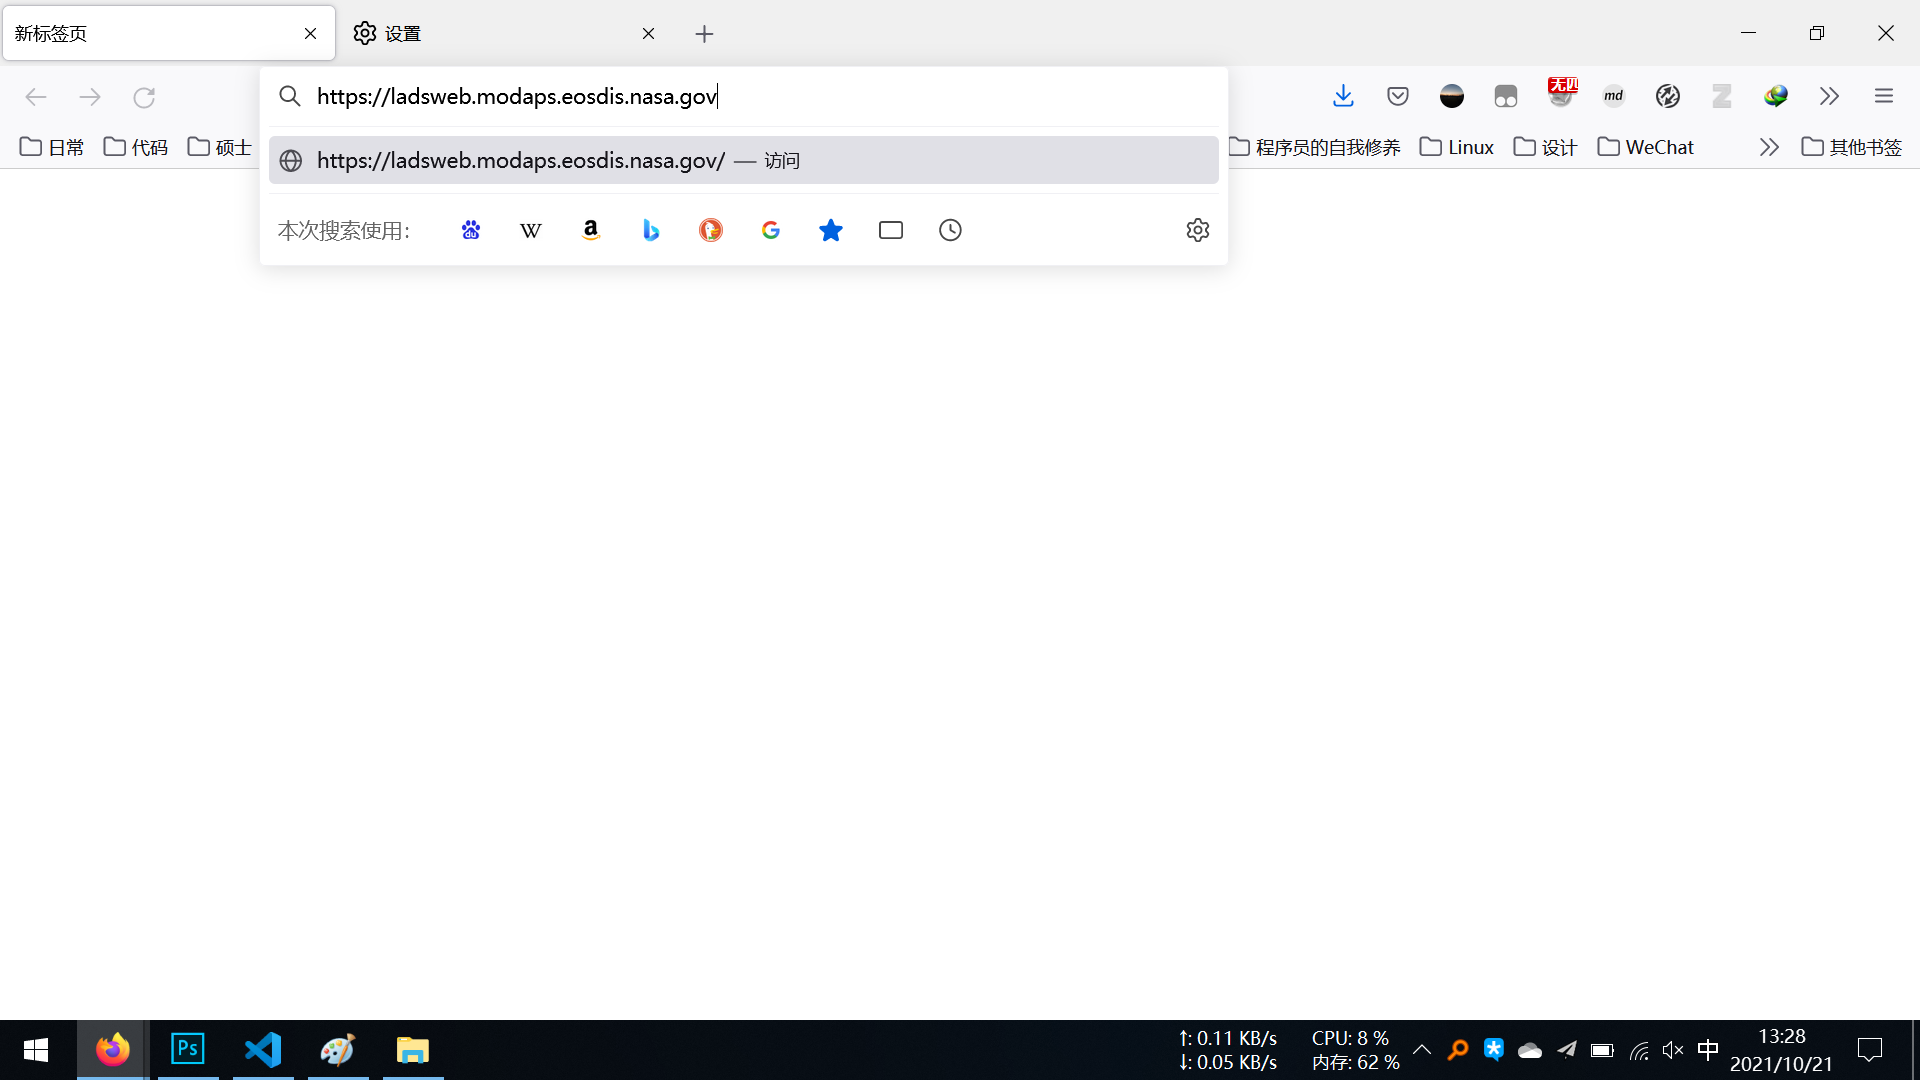
\includegraphics[width=\linewidth]{images/2.输入LAADS网址.png}
\end{frame}
\begin{frame}
    \frametitle{打开登录界面}
    点右上角的\underline{Profile},然后点击 \underline{Earthdata Login}
    \begin{annotationimage}{width=\linewidth}{images/3.找到登录入口.png}
        \draw[red,very thick] (0.855,0.71) -- (0.997,0.71) -- (0.997,0.95) --
        (0.925,0.95) -- (0.925,0.82) -- (0.855,0.82) -- cycle;
    \end{annotationimage}
\end{frame}
%%%% 注册账号 ------------------------------------------------------------------
\subsection{注册帐号}
\begin{frame}
    \frametitle{登录/注册}
    有账号直接输入点 \underline{LOGIN IN}登录,转
    \hyperlink{login}{\beamergotobutton{登录}}

    没帐号点 \underline{REGISTER}注册,转下一页

    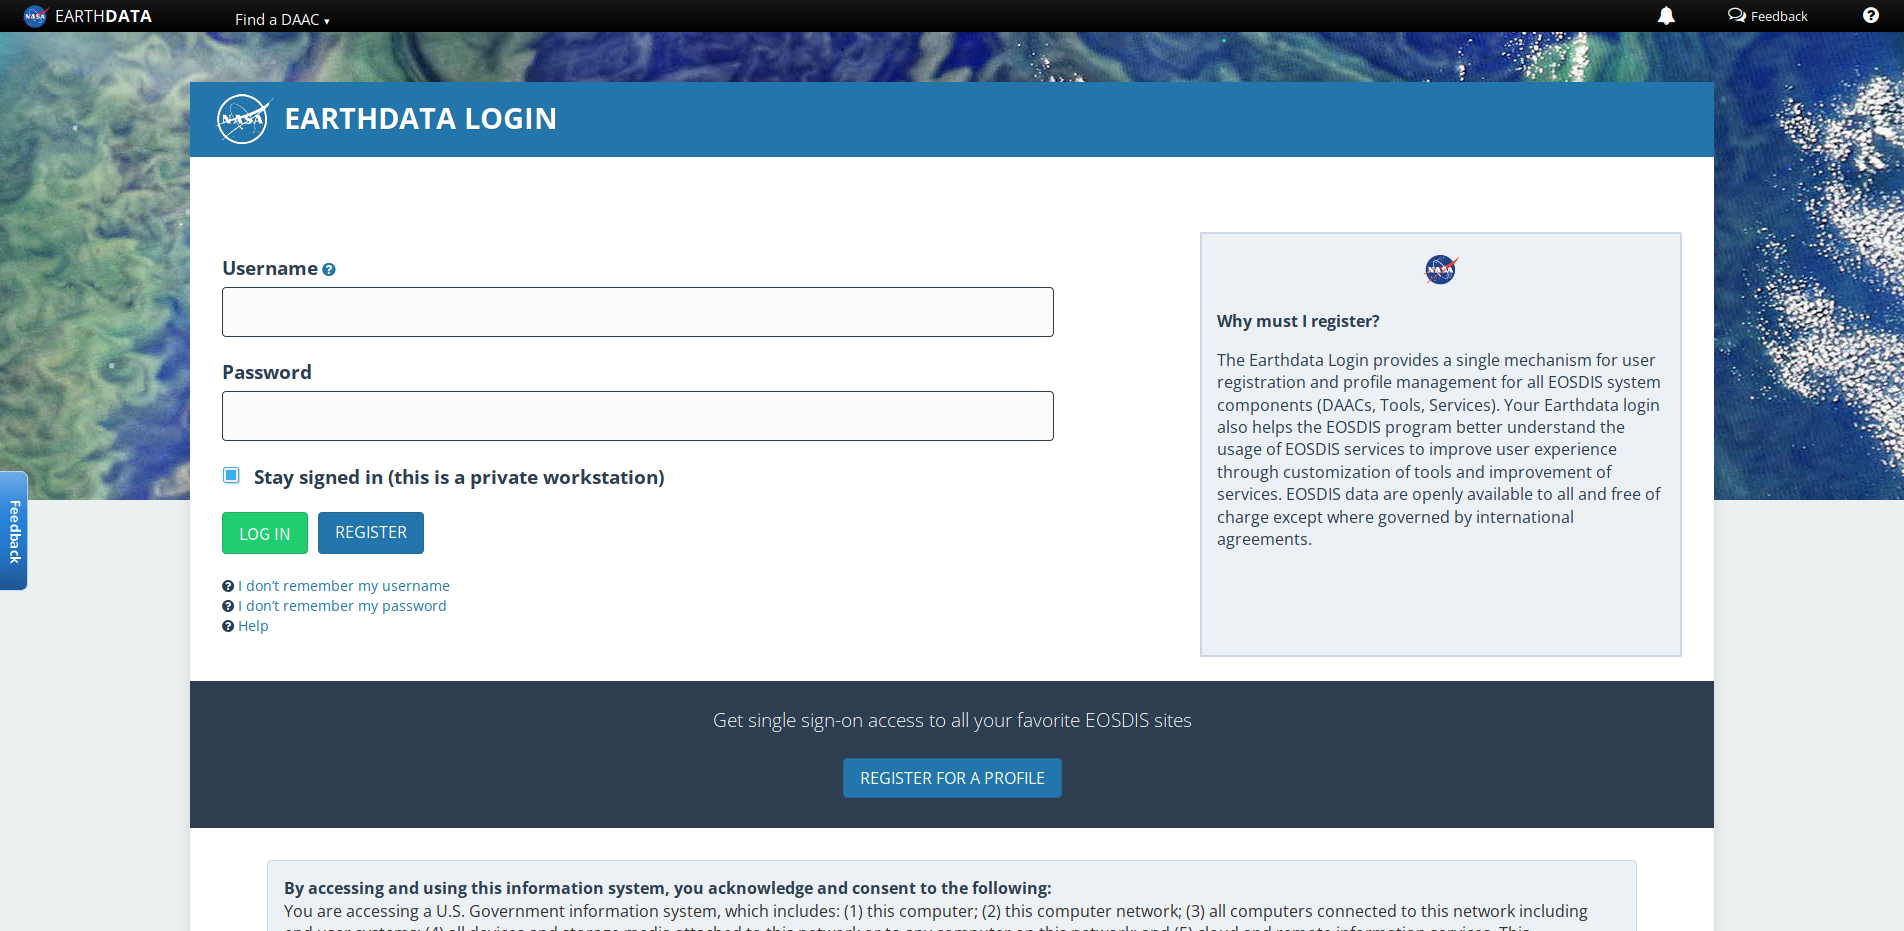
\includegraphics[width=\linewidth]{images/4.登陆界面.png}
\end{frame}
\begin{frame}
    \frametitle{填信息}
    按要求填写标红星的选项
    \footnote{邮箱填QQ邮箱亦可}
    ;底部的Agreements内容全选

    点击底部\underline{Register for Earthdata Login}确认注册
    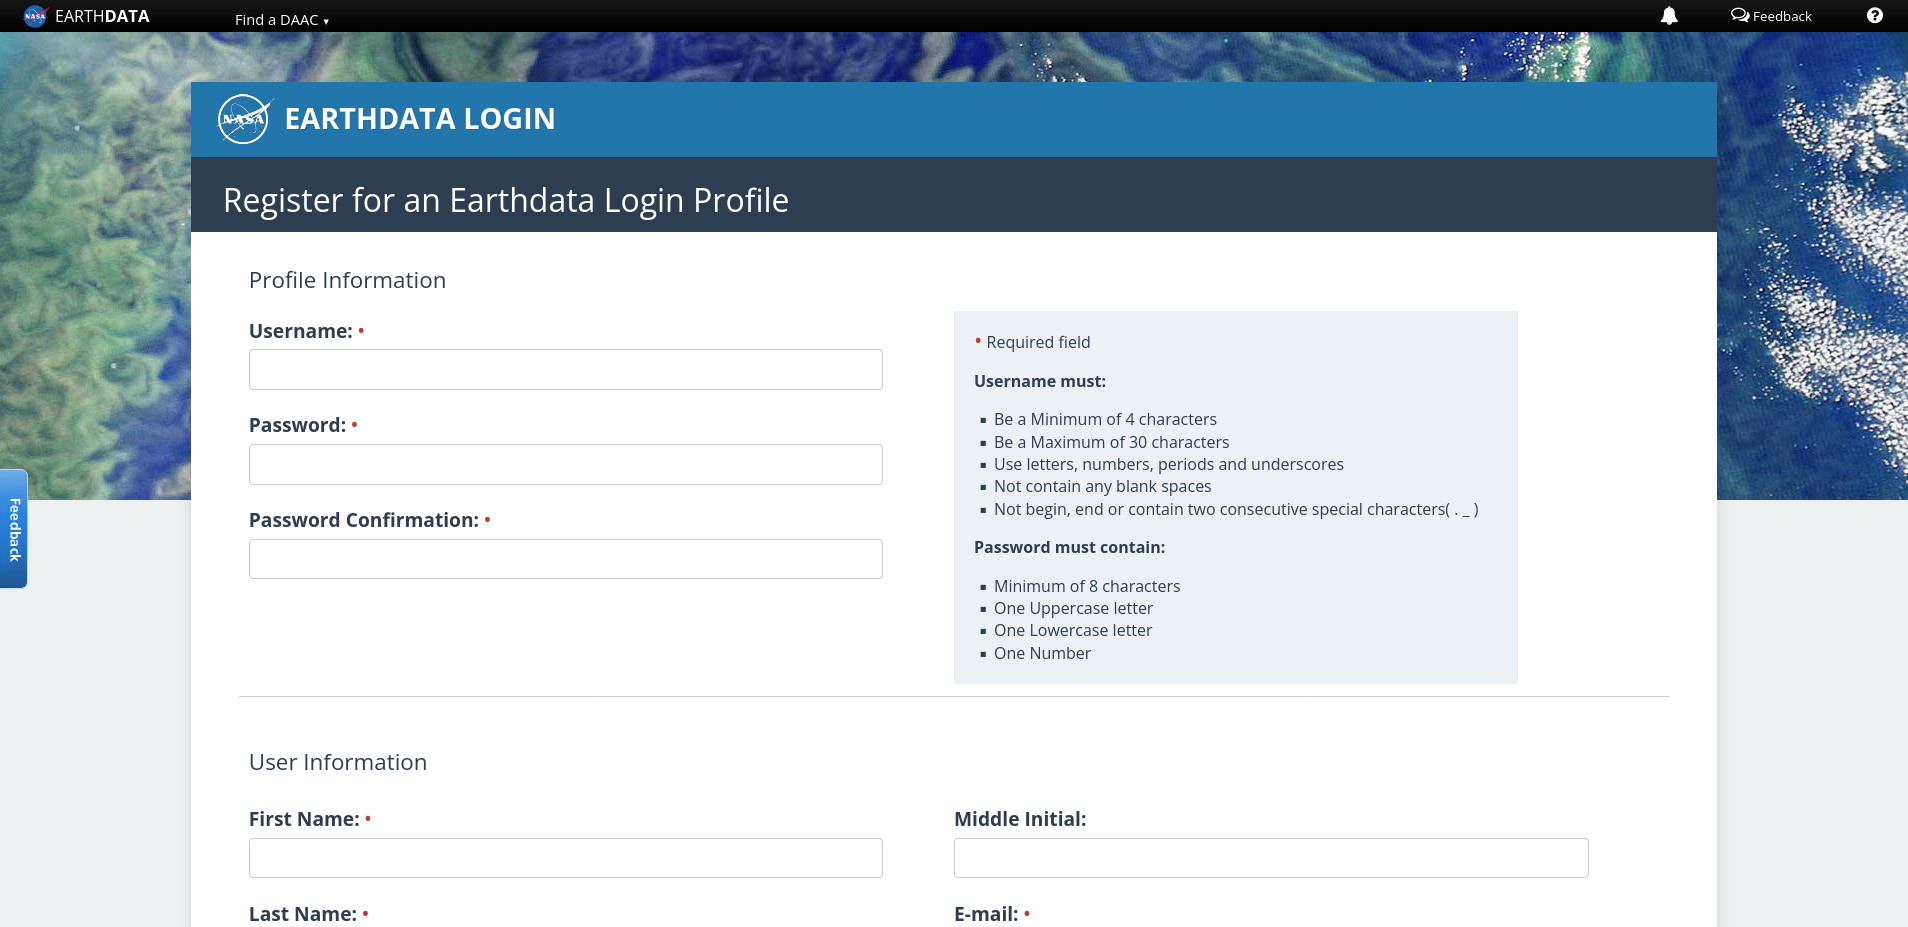
\includegraphics[width=\linewidth]{images/5.注册帐号.png}
\end{frame}
\begin{frame}[label=login]
    \frametitle{登录}
    注册完回来,输入你注册的用户名和密码,登录
    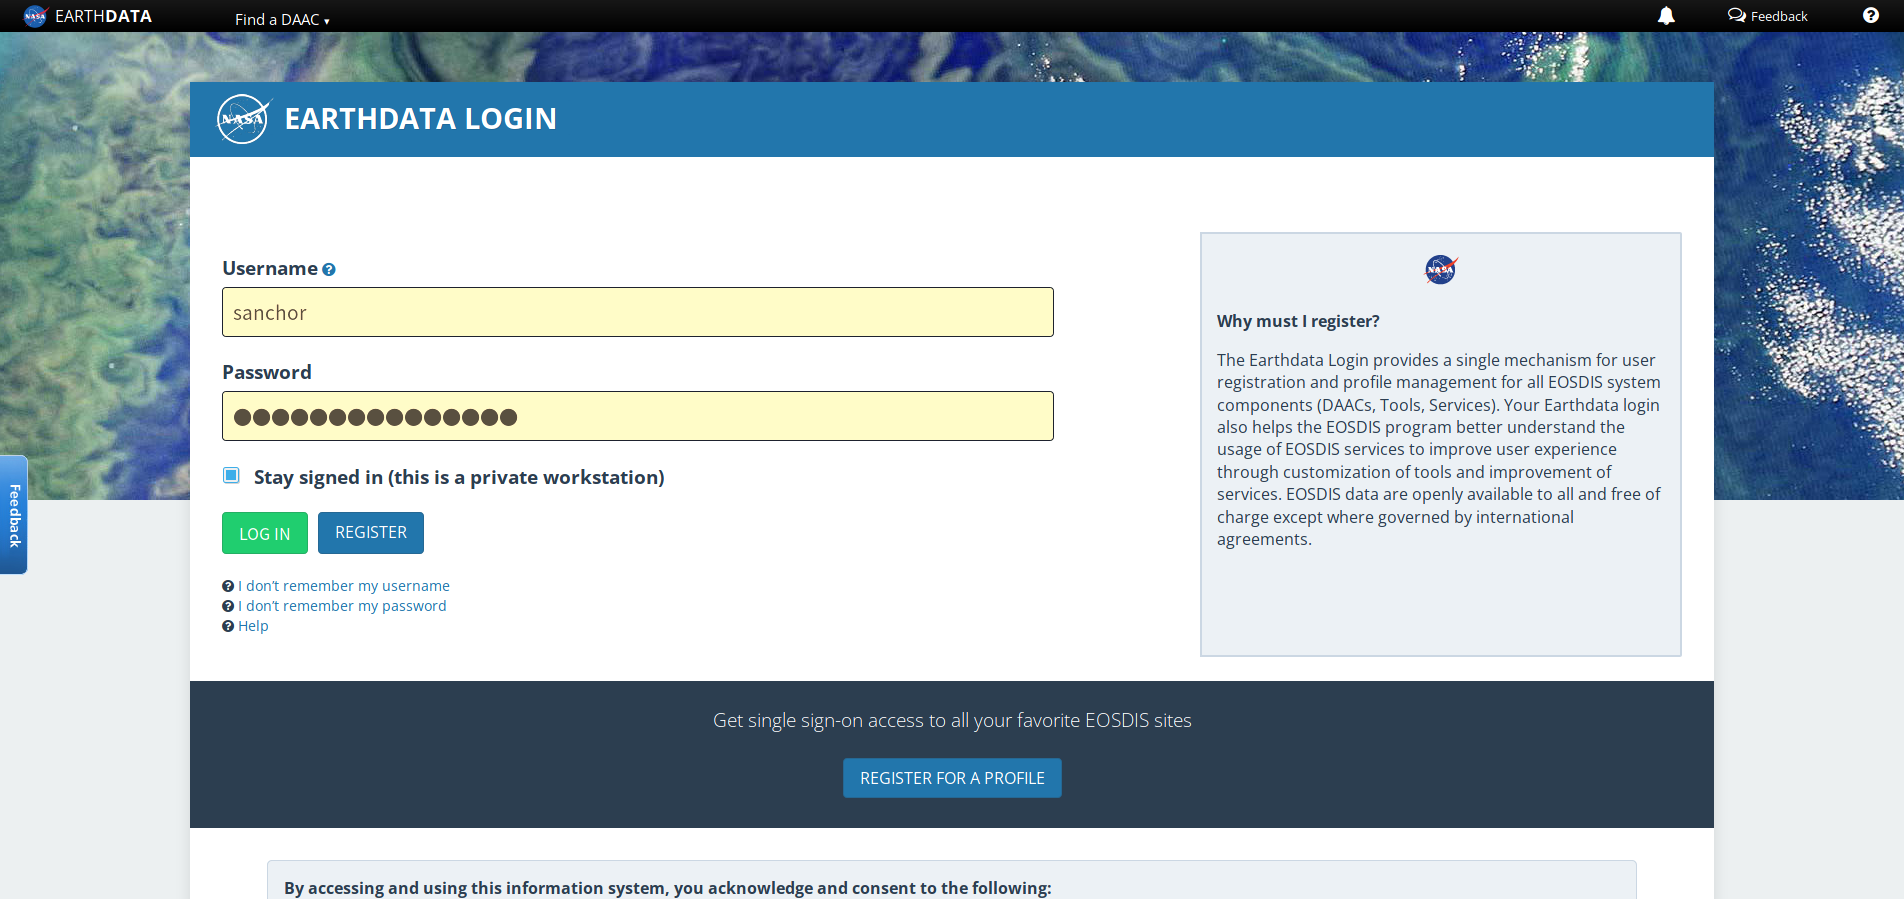
\includegraphics[width=\linewidth]{images/7.登录.png}
\end{frame}
\begin{frame}
    \frametitle{登录完成}
    登录完会返回主页,再点击右上角的 \underline{Profile}会不一样
    \begin{annotationimage}{width=\linewidth}{images/8.登录完成.jpg}
        \draw[red,very thick] (0.87,0.74) -- (0.997,0.74) -- (0.997,0.97) --
        (0.945,0.97) -- (0.945,0.9) -- (0.87,0.90) -- cycle;
    \end{annotationimage}
\end{frame}
%%%% 检索数据 -------------------------------------------------------------------
\subsection{执行检索}
\begin{frame}
    \frametitle{打开检索页面}
    点击主页上的 \underline{Data Discovery},点击 \underline{Find Data}
    \begin{annotationimage}{width=\linewidth}{images/9.找到检索入口}
        \draw[red,very thick] (0.69,0.74) -- (0.84,0.74)-- (0.84,0.96) --
        (0.74,0.96) -- (0.74,0.9) -- (0.69,0.9) --cycle;
    \end{annotationimage}
\end{frame}
\begin{frame}
    \frametitle{选择产品}
    \begin{enumerate}
        \item 左侧分类中选择 \underline{Aerosol}(气溶胶)
        \item 右侧气溶胶产品中选择AERDT\_L2\_VIIRS\_SNPP
    \end{enumerate}
    \begin{annotationimage}{width=\linewidth}{images/10.选择产品}
        \draw[red,very thick] (0.06,0.38) rectangle (0.34,0.42);
        \draw[red,very thick] (0.38,0.51) rectangle (0.96,0.57);
        \draw[coordinate label = {1 at (0.2,0.4)}];
        \draw[coordinate label = {2 at (0.67,0.54)}];
    \end{annotationimage}
\end{frame}
\begin{frame}
    \frametitle{设置日期范围}
    \begin{enumerate}
        \item 点击 \underline{TIME},进入时间选择界面
        \item 如图设置时间范围
    \end{enumerate}
    \begin{annotationimage}{width=\linewidth}{images/11.选择日期}
        \draw[red,very thick] (0.28,0.88) rectangle (0.44,0.94);
        \draw[red,very thick] (0.17,0.64) rectangle (0.36,0.7);
        \draw[coordinate label = {1 at (0.25,0.91)}];
        \draw[coordinate label = {2 at (0.14,0.67)}];
    \end{annotationimage}
\end{frame}
\begin{frame}
    \frametitle{添加日期}
    点击\underline{Add Date},所选日期范围就会在右侧列表中显示
    \begin{annotationimage}{width=\linewidth}{images/12.添加日期}
        \draw[red,very thick] (0.2,0.6) rectangle (0.325,0.645);
        \draw[red,very thick] (0.53,0.7) rectangle (0.92,0.8);
    \end{annotationimage}
\end{frame}
\begin{frame}
    \frametitle{设置空间范围}
    \begin{enumerate}
        \item 点击 \underline{LOCATION},进入区域选择界面
        \item 点击 \underline{Countries},按照国界选择范围。点击中国区域即为选中
    \end{enumerate}
    \begin{annotationimage}{width=\linewidth}{images/13.选择区域}
        \draw[red,very thick] (0.44,0.88) rectangle (0.59,0.94);
        \draw[red,very thick] (0.83,0.69) rectangle (0.98,0.75);
        \draw[coordinate label = {1 at (0.41,0.91)}];
        \draw[coordinate label = {2 at (0.95,0.72)}];
    \end{annotationimage}
\end{frame}
\begin{frame}
    \frametitle{选中检索结果}
    \begin{enumerate}
        \item 点击 \underline{FILES},进入文件检索界面
        \item 待检索文件数目稳定后,点击 \underline{Select All}全部选中
    \end{enumerate}
    \begin{annotationimage}{width=\linewidth}{images/14.检索文件}
        \draw[red,very thick] (0.59,0.88) rectangle (0.74,0.94);
        \draw[red,very thick] (0.38,0.76) rectangle (0.44,0.82);
        \draw[coordinate label = {1 at (0.56,0.91)}];
        \draw[coordinate label = {2 at (0.35,0.79)}];
    \end{annotationimage}
\end{frame}
%%%% 提交查看订单 ---------------------------------------------------------------
\subsection{查看订单}
\begin{frame}
    \begin{enumerate}
        \item 点击 \underline{REVIEW \& OEDER},进入订单提交界面
        \item 确认无误后点击 \underline{Submit Order},提交订单
    \end{enumerate}
    \frametitle{提交订单}
    \begin{annotationimage}{width=\linewidth}{images/15.提交订单}
        \draw[red,very thick] (0.73,0.88) rectangle (0.92,0.94);
        \draw[red,very thick] (0.78,0.56) rectangle (0.96,0.62);
        \draw[coordinate label = {1 at (0.70,0.91)}];
        \draw[coordinate label = {2 at (0.75,0.59)}];
    \end{annotationimage}
\end{frame}
\begin{frame}
    \frametitle{已提交订单}
    订单已提交,可以点击 \underline{Click here to continue}返回起始位置。
    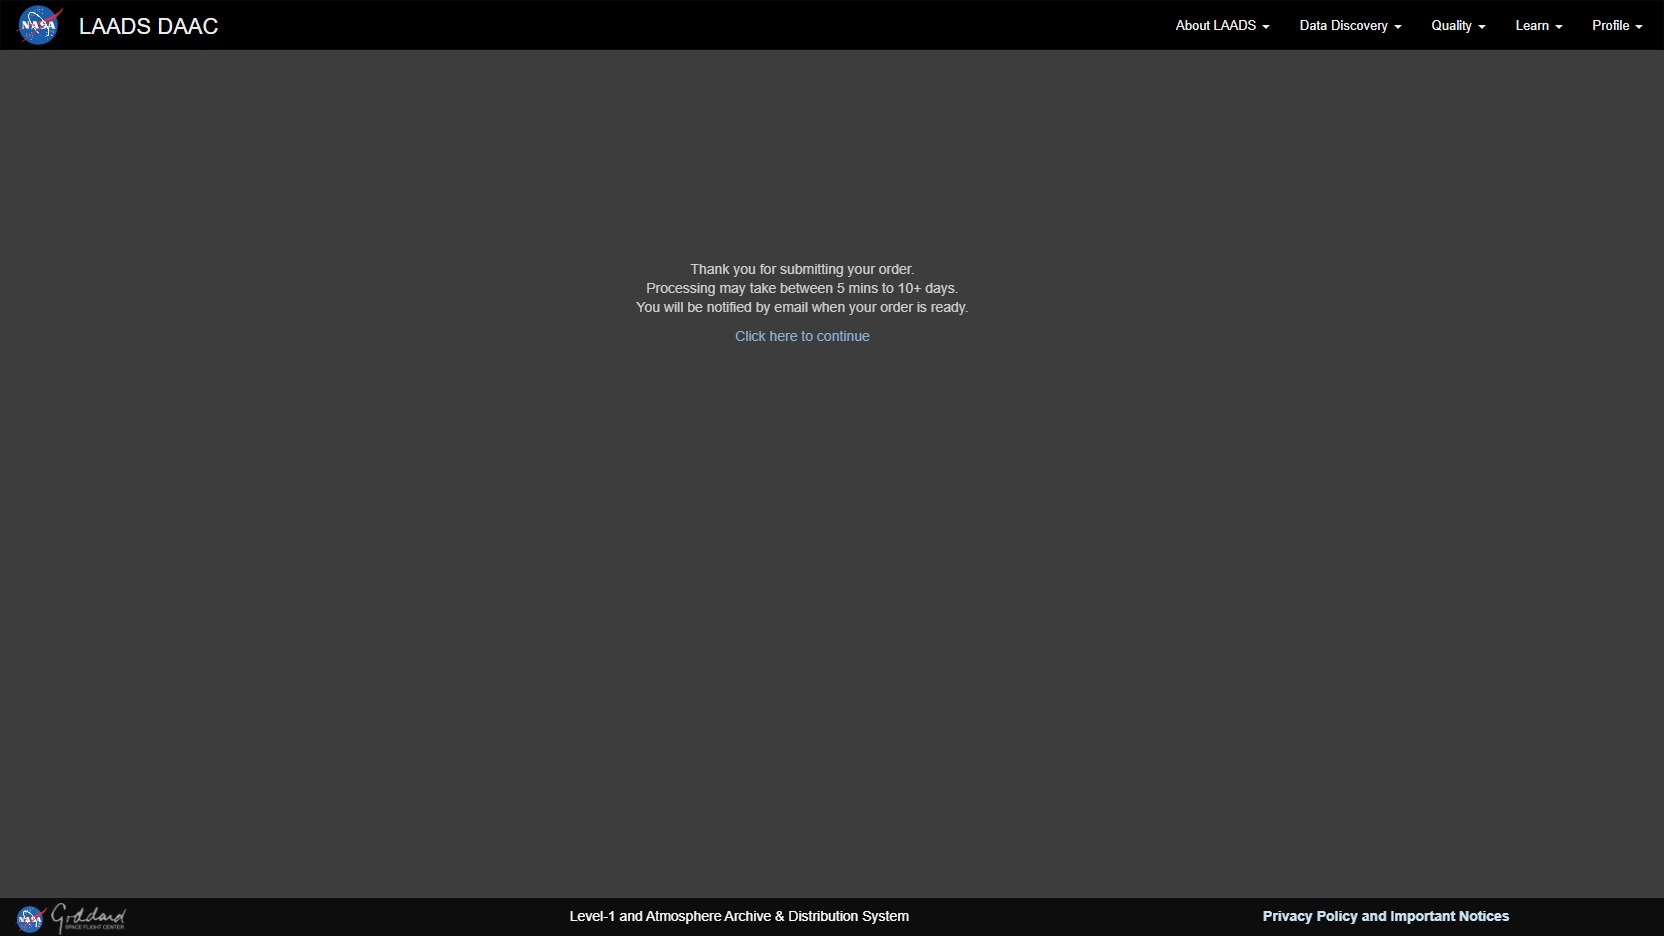
\includegraphics[width=\linewidth]{images/16.已提交订单}
\end{frame}
\begin{frame}
    \frametitle{查看历史订单}
    点击\underline{Past Orders},进入历史订单界面
    \begin{annotationimage}{width=\linewidth}{images/17.回到起始点}
        \draw[red,very thick] (0.001,0.44) -- (0.045,0.44) -- (0.045,0.52) --
        (0.001,0.52);
    \end{annotationimage}
\end{frame}
\begin{frame}
    \frametitle{历史订单}
    当历史订单条目显示绿色时,说明该订单已准备就绪,是可下载状态,注意有Available字样
    \begin{annotationimage}{width=\linewidth}{images/18.历史订单列表}
        \imagelabelset{image label back = white,image label text = black}
        \draw[image label = {为了保护密集恐惧症患者,其余历史订单条已被遮挡 at south}];
    \end{annotationimage}
    

\end{frame}
\begin{frame}
    \frametitle{查看订单内容}
    打开订单内容,看看是否真的准备好了
    \begin{annotationimage}{width=\linewidth}{images/19.展开订单}
        \draw[red,very thick](0.28,0.74) rectangle (0.4,0.78);
    \end{annotationimage}
\end{frame}
\begin{frame}
    \frametitle{订单内容}
大功告成,准备下载吧!
    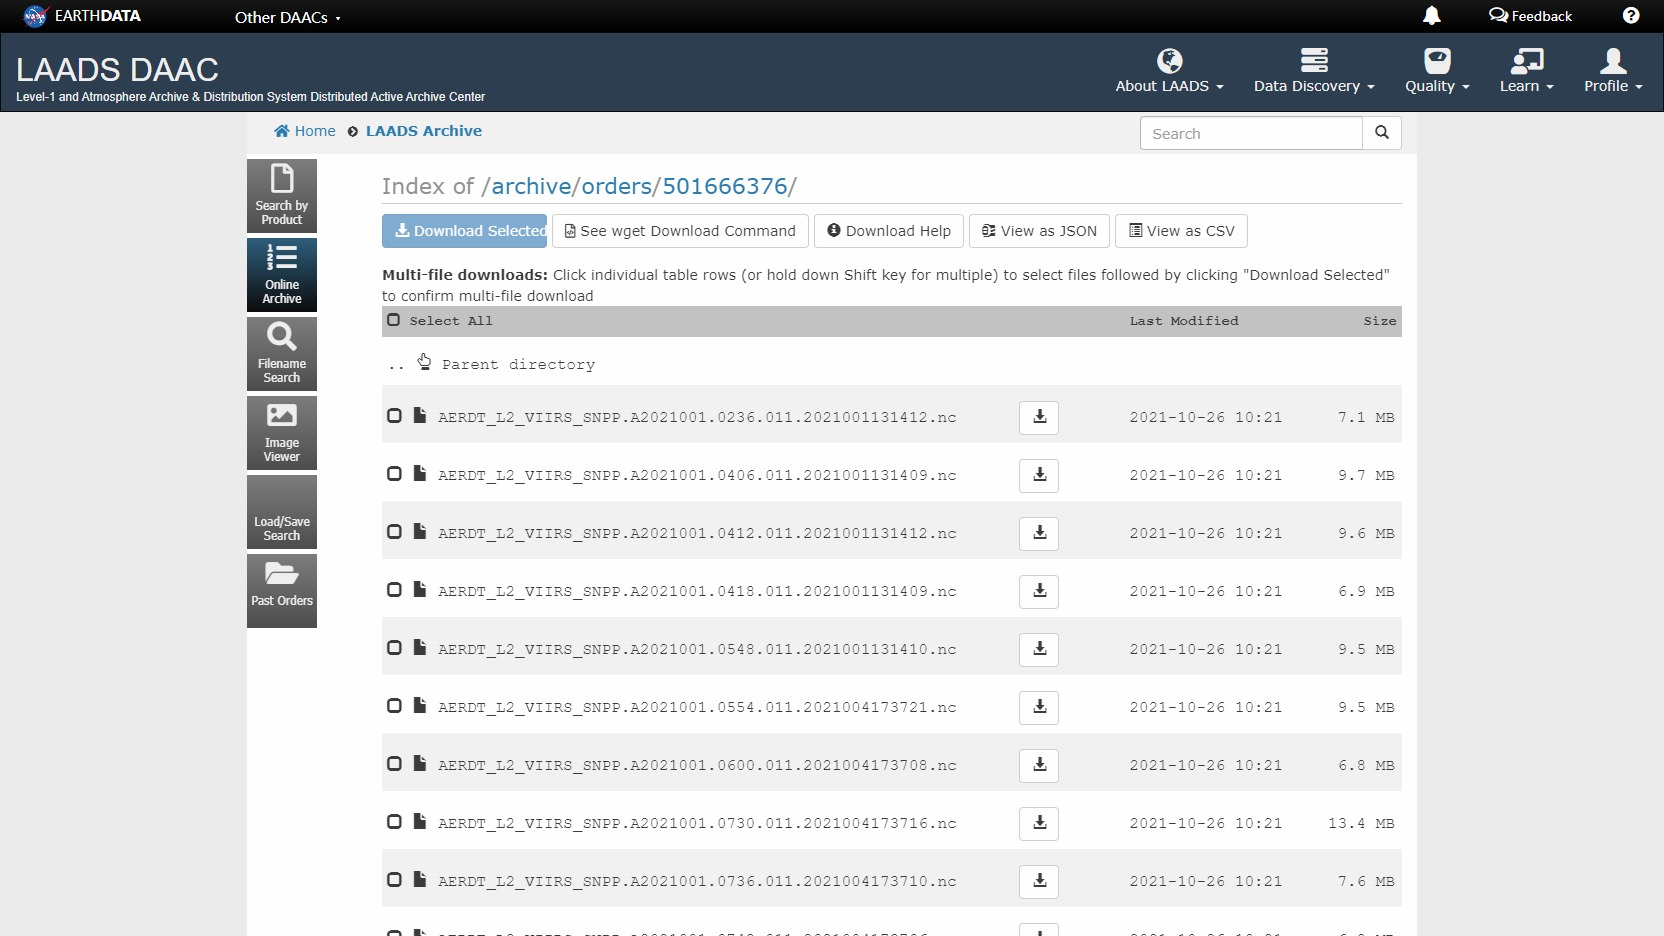
\includegraphics[width=\linewidth]{images/20.订单内容}
\end{frame}